%--------------------------------------------%
% Template Beamer para Apresentações da UFRN %
% by alcemygvseverino@gmail.com              %
% Baseado em MIT Beamer Template			 %
% versao 1.1								 %
% Atualizado em 14/05/2016					 %
%--------------------------------------------%
\documentclass[handout]{beamer}
% Para alterar a linguagem do documento
\usepackage[portuges]{babel}
% Para aceitar caracteres especias deretamente do teclado
\usepackage[utf8]{inputenc}
% Para seguir as normas da ABNT de citacao e referencias
\usepackage[alf]{abntex2cite}
% Para incluir figuras
\usepackage{graphicx}
% Para melhor ajuste da posisao das figuras
\usepackage{float}
% Para ajustar as dimensoes do layout da pagina
\usepackage{geometry}
% Para formatar estrutura e informacoes de formulas matematicas
\usepackage{amsmath}
% Para incluir simbolos especiais em formulas matematicas
\usepackage{amssymb}
% Para incluir links nas referencias
\usepackage{url}
% Para incluir paginas de documentos .pdf externos
\usepackage{pgfpages}
% Para ajustar o estilo dos contadores
\usepackage{enumerate}
% Para modificar a cor do texto
\usepackage{color}
% Para incluir condicoes
\usepackage{ifthen}
% Para colocar legendas em algo que nao e float
\usepackage{capt-of}
% Para definir o tema do slide
\usetheme{Berlin}

\usepackage{minted}
\definecolor{blcodebg}{rgb}{0.9,0.9,0.9}

% Para difinir cores e background
\usecolortheme{ufrn}
% Para numerar as figuras
\setbeamertemplate{caption}[numbered]
\usepackage{caption}
\renewcommand{\thefigure}{\hspace{-.333333em}}
% Título
\title[Trabalho de conclusão de curso]{
	Implementação do sistema de arquivos SquashFS no bootloader U-Boot}
% Data
\date{
	\today}
% Autores
\author[João Marcos Correia de Lima Costa]{
	João Marcos Correia de Lima Costa %\inst{1}\\
	%\vspace{0.25cm}
	%Autor 02 \inst{2}}
	}
% Instituto
\institute[INSTITUTO]{
	%\inst{1}%
	%\url{jmcosta944@mail.com}\\
	\vspace{0.25cm}
	%\inst{2}%
	Departamento de Engenharia Elétrica\\
	Universidade Federal do Rio Grande do Norte}
% Logo do canto inferior direito
\pgfdeclareimage[height=0.7cm]{logo_UFRN}{figuras/logo_UFRN}
\logo{
	\vspace*{-0.25cm}
	\pgfuseimage{logo_UFRN}
	\hspace*{-0.05cm}}


\begin{document}
% Sumário
\frame{\titlepage}
%\section[]{}
\begin{frame}{Sumário}
	\tableofcontents
\end{frame}
% Introducao

\section{Introdução}
\begin{frame}{Introdução}
	A Introdução vai aqui
\end{frame}


% Metodologia
\section{Metodologia}
\begin{frame}{Metodologia}
	Metodologia aqui.
\end{frame}

% Resultados
\section{Resultados}
\begin{frame}[fragile]{Resultados}
Console do U-Boot, lançado na Beagle Bone Black Wireless:
\begin{minted}[fontsize=\fontsize{4}{4}, bgcolor=blcodebg]{text}
U-Boot SPL 2020.10-rc1-00154-gc7b2d6a45d (Aug 07 2020 - 11:17:02 +0200)
Trying to boot from MMC1

U-Boot 2020.10-rc1-00154-gc7b2d6a45d (Aug 07 2020 - 11:17:02 +0200)

CPU  : AM335X-GP rev 2.1
Model: TI AM335x BeagleBone Black
DRAM:  512 MiB
WDT:   Started with servicing (60s timeout)
NAND:  0 MiB
MMC:   OMAP SD/MMC: 0, OMAP SD/MMC: 1
Loading Environment from FAT... Unable to use mmc 0:1... <ethaddr> not set.
Validating first E-fuse MAC
Net:   Could not get PHY for ethernet@4a100000: addr 0
eth2: ethernet@4a100000, eth3: usb_ether
Hit any key to stop autoboot:  0
=> sqfsls mmc 0:1
            bin/
            boot/
            dev/
            etc/
            lib/
    <SYM>   lib32
    <SYM>   linuxrc
            media/
            mnt/
            opt/
            proc/
            root/
            run/
            sbin/
            sys/
            tmp/
            usr/
            var/

2 file(s), 16 dir(s)
\end{minted}
\end{frame}

\begin{frame}[fragile]{Resultados}
Carregando o kernel e a device tree:
\begin{minted}[fontsize=\fontsize{7}{7}, bgcolor=blcodebg]{text}
=> sqfsload mmc 0:1 $kernel_addr_r /boot/zImage
6091376 bytes read in 476 ms (12.2 MiB/s)
=> sqfsload mmc 0:1 $fdt_addr_r /boot/am335x-boneblack.dtb
40817 bytes read in 14 ms (2.8 MiB/s)
=> setenv bootargs console=ttyO0,115200n8
=> bootz $kernel_addr_r - $fdt_addr_r
## Flattened Device Tree blob at 81000000
   Booting using the fdt blob at 0x81000000
   Loading Device Tree to 8fff3000, end 8fffff70 ... OK

Starting kernel ...

[    0.000000] Booting Linux on physical CPU 0x0
[    0.000000] Linux version 4.19.79 (joaomcosta@joaomcosta-Latitude-E7470)
(gcc version 7.3.1 20180425 [linaro-7.3-2018.05 revision
d29120a424ecfbc167ef90065c0eeb7f91977701] (Linaro GCC 7.3-2018.05))
#1 SMP Fri May 29 18:26:39 CEST 2020
[    0.000000] CPU: ARMv7 Processor [413fc082] revision 2 (ARMv7), cr=10c5387d
\end{minted}
\end{frame}


\begin{frame}{Resultados}
\begin{itemize}
\item O suporte do SquashFS foi aceito e integrado ao código oficial do U-Boot
\begin{figure}
\centering
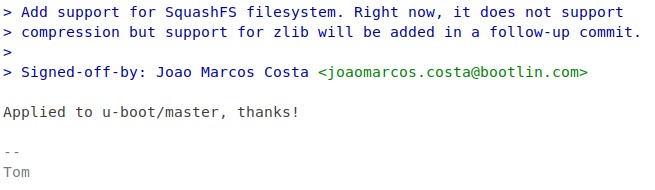
\includegraphics[scale=0.4]{figuras/tom.jpeg}
\caption{Mensagem de aceite de Tom Rini, administrador principal do U-Boot}
\end{figure}
\item Balanço final: 27 arquivos novos e/ou modificados e aproximadamente 3000 linhas de código
\end{itemize}
\end{frame}


% Conclusao
\section{Conclusão}
\begin{frame}{Conclusão}
	\begin{itemize}
	    \item Algoritmos de compressão suportados: LZO, GZIP e ZSTD.
	    \item Contribuições recorrentes por parte da comunidade (internacional) do U-Boot
	    \item Otimizações de seções do código
	    \item Contribuições paralelas à documentação não-oficial usada como referência
	\end{itemize} 
\end{frame}

% Referencias
\section{Referencias}
\begin{frame}{Referências}
	Suas referencias bibliográficas aqui, siga o modelo ABNT.
	\bibliography{bib/bibliografia}
\end{frame}

% Agradecimentos
\section{}
\begin{frame}{Agradecimentos}
	Agradeço a todos. 	
\end{frame}

\end{document}